\subsection{Supervised Learning}

\textbf{Supervised Learning} is the task of 'learning' a function relationship, based on a given set of inputs/outputs.

Some terminology:

\begin{tabular}{ll}
    $x \in \R^d$                    & Inputs (Attributes/Covariates)    \\
    $\phi(x) \in \R^p$              & Features                          \\
    $y \in \R$                      & Outputs (Targets/Labels)          \\
    $D = \{ (x_i,y_i) \}_{i=1}^n$   & Training Set                      \\
    $D'$                            & Test Set                          \\
    $f: \R^p \to \R$                & Predictor (Model)                 \\
    $l(f(x), y)$                    & Loss                  
\end{tabular}

\textbf{Machine Learning Pipelines} can often be classified using:

\begin{tabular}{ll}
    $F$                             & Function Class                    \\
    $L(f)$                          & Training Loss                     \\
                                    & Optimization Method
\end{tabular}

{\small
    The function class $F$ is a set of parametrized functions. 
    We are looking for the $f \in F$ that minimizes $L(f)$.
}

\definition \textbf{Training Loss}
$$
    L(f) := \frac{1}{n}\sum_{i=1}^{n} l\bigl( f(x_i), y \bigr) 
$$

\newpage

\subsection{Multiple Linear Regression}

\textbf{Multiple Linear Regression} directly uses the $x \in \R^d$. \\
Here, $F_\text{affine} = \bigl\{ f(x) = w^\top x + w_0 \big| w \in \R^d, w_0 \in \R \bigr\}$. 

\remark Why are we using linear functions instead?\\
{\footnotesize\color{gray}
    Any estimator $f \in F_\text{affine}$ can be rewritten as $f\bigl((x,1)\bigr) = (w,w_0)^\top\cdot(x,1)$,
    thus we can augment the inpurs $x \mapsto (x,1)$ and \\
    instead search in $F_\text{linear} = \{ f(x) = \hat{w}^\top x | \hat{w} \in \R^{d+1} \}$
}

\subsection{Loss Functions}

\definition \textbf{Squared Loss} $\quad l\bigl( f(x),y \bigr) := \bigl( f(x) - y \bigr)^2$\\
\subtext{Most common Loss Function, but sensitive to outliers.}

\definition \textbf{Absolute Loss} $\quad l_\text{abs}\bigl( f(x),y \bigr) := |f(x)-y|$\\
\subtext{Less sensitive to outliers, but not differentiable.}

\definition \textbf{Huber Loss}
$$
    l_\text{huber}\bigl( f(x),y \bigr) := \begin{cases}
        \frac{1}{2}\bigl( f(x)-y \bigr)^2                   & |f(x)-y| \leq \delta \\
        \delta \bigl( |f(x)-y| - \frac{1}{2}\delta \bigr)   & |f(x)-y| > \delta
    \end{cases}
$$
\subtext{Using parameter $\delta$, the penalization of outliers can be controlled}

\textbf{Assymetric Loss}: In some cases it is desirable to penalize overestimation harder than underestimation, or vice versa.

\definition \textbf{Quantile Loss}
$$
    l_\tau\bigl( f(x),y \bigr) := \tau \max\Bigl\{ y-f(x),0 \Bigr\} + (1-\tau)\max\Bigl\{ f(x)-y, 0 \Bigr\}
$$
\subtext{Using parameter $\tau$, over/underestimation can be penalized}

\newpage

\subsection{The Normal Equation}
The normal equation is the basis for the closed form solution of linear regression. (square loss)

To find $\hat{f} := \underset{f \in F_\text{linear}}{\text{arg min}} L(f)$ we look for ideal weights $\hat{w} \in \R^d$.
$$
    \hat{w} := \underset{w \in \R^d}{\text{arg min}} L(f_w) = \frac{1}{n}\sum_{i=1}^{n}\underbrace{\Bigl( y_i - w^\top x_i \Bigr)^2}_{l\bigl(f(x_i), y_i\bigr)}
$$
\subtext{A natural abuse of notation here is $L(w) := L(f_w)$.}

This can be rewritten in matrix notation:
$$
    \sum_{i=1}^{n}\Bigl( y_i - w^\top x_i \Bigr)^2 = \bigl\Vert y-Xw \bigr\Vert^2
$$
\subtext{The factor $\frac{1}{n}$ is irrelevant for Optimization, it doesn't depend on $w$}

So we find a problem familiar from linear algebra:
$$
    \hat{w} = \underset{w \in \R^d}{\text{arg min}} \bigl\Vert y-Xw \bigr\Vert^2
$$
The solution is a stationary point, so:
$$
    \nabla_w \bigl\Vert y-Xw \bigr\Vert^2 = 2X^\top(X\hat{w}-y) \overset{!}{=} 0
$$
Which yields the \textbf{Normal Equation}.
$$
    \mathbf{X}^\top\mathbf{X}\hat{w} = \mathbf{X}^\top y
$$

\theorem \textbf{Geometric Interpretation}\\
$\hat{y} = \mathbf{X}\hat{w}$ for $\hat{w}$ solving $\mathbf{X}^\top\mathbf{X}\hat{w} = \mathbf{X}^\top y$ is the orthogonal projection of $y$ onto $\text{span}(\mathbf{X})$.

\begin{center}
    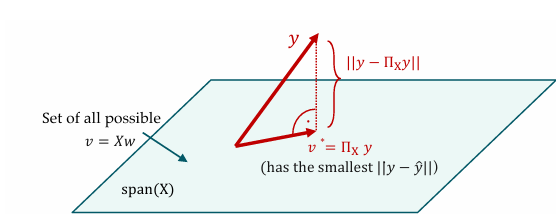
\includegraphics[width=0.275\textwidth]{resources/normalEquation.png}\\
    \subtext{Introduction to Machine Learning (2026), p. 74}
\end{center}

\newpage

\subsection{Closed Form Solution}

\theorem \textbf{Minimum-Norm Solution}\\
$$
    \hat{w} = \Bigl(\mathbf{X}^\top\mathbf{X}\Bigr)^\dagger\mathbf{X}^\top y = \mathbf{X}^\top\Bigl(\mathbf{X}^\top\mathbf{X}\Bigr)^{-1} \mathbf{X}^\top y 
$$
$$
    \text{for} \qquad \hat{w} = \underset{w \in \R^d}{\text{arg min}} \bigl\Vert w \bigr\Vert^2
$$

{\footnotesize
    \remark The computational cost for this is $\mathcal O (nd^2+d^3)$.
}

The closed form solution depends on $\text{rank}(\mathbf{X})$.

Assuming $d \leq n$ and $\text{rank}(\mathbf{X}) = d$: $(\mathbf{X}^\top\mathbf{X})^{-1}$ exists.
$$
    \hat{w} = (\mathbf{X}^\top\mathbf{X})^{-1}\mathbf{X}^\top y \qquad (\text{unique})
$$
Assuming $d > n$ or $\text{rank}(\mathbf{X}) < d$ we have $|\ker(\mathbf{X})|=\infty$ and there are infinite solutions. The pseudo-inverse provides the minimum-norm solution:
$$
    \hat{w} = \Bigl(\mathbf{X}^\top\mathbf{X}\Bigr)^\dagger \mathbf{X}^\top y
$$
{\footnotesize
    \remark If $\text{rank}(\mathbf{X})=d$, then $\bigl(\mathbf{X}^\top\mathbf{X}\bigr)^\dagger = \bigl(\mathbf{X}^\top\mathbf{X}\bigr)^{-1}$.
}

\subsection{Non-Linear Least Squares}

To expand Linear Regression to Non-linear functions, feature maps are used on $x$: $\phi: \R^d \to \R^p$.
$$
    f_w(x) = \sum_{j=1}^{p} w_j^\top \phi_j(x)
$$
This induces a function class different from $F_\text{linear}$:
$$
    F_\phi = \biggl\{ f_w(x) = \sum_{j=1}^{p} w_j^\top \phi_j(x) \ \bigg|\ w \in \R^p \biggr\}
$$
But the optimization problem remains the same:\\
\subtext{$\Phi \in \R^{n \times p}$ now replaces $\mathbf{X} \in \R^{n \times d}$.}
$$
    \hat{w} = \underset{w\in\R^p}{\text{arg min}} \Bigl\Vert y - \Phi w \Bigr\Vert^2
$$

\begin{center}
    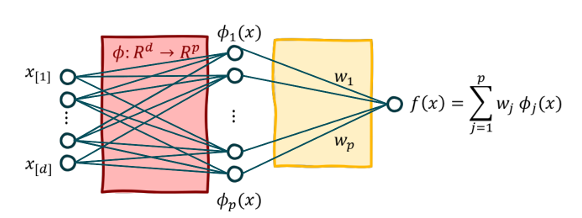
\includegraphics[width=0.2\textwidth]{resources/nonlinearLeastSquares.png}\\
    \subtext{Introduction to Machine Learning (2026), p. 79}
\end{center}